\chapter{Some Big Ideas}

\centering

\includegraphics{../images/book-5104342_1920.jpg}

\justify{}
There are some key precepts that will serve the aspiring DevSecOps engineer well. In this
chapter we will explore some of these in an attempt to level-set our understanding of the
domain. We will also continue to introduce the reader to the vernacular of the modern day
DevSecOps engineer in a world gone cloudy. You certainly don't need to memorize all of 
these terms, but the thinking is they are prevalent enough that you should have a passing 
familiarity with them. 

\section{Revision Control}

\justify{}
Code, documents, test cases, and other software work products begin their lives on the workstations of creators
and developers. In this book we will refer to the environments where this takes place as the ``local'' environment.
These work products are typically created, reviewed and checked into Revision Control Systems 
(RCS)\index{Revsion Control System (RCS)}, GitHub\index{GitHub} for example, by the DevSecOps practitioner. 
Other popular revision control systems include GitLab\index{GitLab} and BitBucket\index{BitBucket}.

\justify{}
Although it may seem like there are a lot of choices when it comes to revision control, there is one tool that
underlies them all. That tool is known as git. Git is the brainchild of Linus Torvalds, who also happens to be
the person that invented the Linux kernel just before the turn of the century. This tool work wonderfully on projects small
and large. For this and may other reasons, it is at the heart of many of these RCS systems that we just mentioned. Note that
in addition to these websites, there are many desktop tools meant to aid developers with revision control on their local
machine. While these can be quite handy, there is no substitute for learning the intricacies of git from the command
line. It will come in quite handy indeed.

We will look more closely at git and revision control in a later chapter.

\section{Testing}

\justify{}
We will delve into various types and aspects of testing throughout this book. For now it is enough to understand the idea of
a test case as a discrete check, or grouping of similar types of checks, that we use to ensure our work products meet
certain minimum standards.  Test cases are created with and often run against our work products at the time they are checked
in to the revision control system. This is meant to ensure stability, security, and compatibility
with the existing code base in revision control. The automation required to execute tests every time work is checked in to
revision control is typically the responsibility of the DevSecOps engineers.

\section{Pipelines}

\begin{figure}[!htb]
\centering
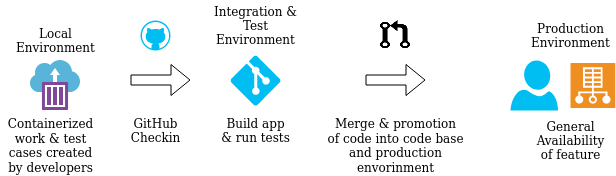
\includegraphics[scale=0.63]{../images/flow.png}
\caption{Typical build pipeline}
\label{pipeline}
\end{figure}

\justify{}
As seen in figure\ref{pipeline}, work typically flows from the local environments, into a test environment, and finally to production
where it is available for use by the entire user base.

\justify{}
We will refer to the entirety of this three-stage flow as one example of what is known as a build pipeline\index{pipeline}.
Code from one or more local environments is checked in to the revision control system throughout a
typical DevSecOps workday, and continuously tested and integrated with the main code base. That is to say, work undergoes
Continuous Integration (CI)\index{Continuous Integration (CI)} with the main code base,
and often Continuous Delivery (CD)\index{Continuous Delivery (CD)} between local, test, and production environments. This is
where the term ``CI/CD Pipeline'' comes from. A business unit may choose to designate more than just the three dev, test,
and prod environments mentioned here, depending on their particular use cases and ways of working.

\justify{}
While the CI/CD Pipeline is often a primary focus of the DevSecOps engineer, other pipelines exist as well. For example,
let's assume our organization maintains a vast pool of raw data, also known as a data lake\index{Data Lake}. The staff Data
Engineers build and maintain Data Science\index{Data Science} pipelines to facilitate the smooth flow
of logs and other data into that data lake. Now Data Scientists are able to create machine learning models that rely on that
data to produce useful insights. As another example, consider code changes as they move from
developer workstations into a code repository for storage. Accessing this code for the purpose of testing will differ from
how it is accessed for the purposes of deployment. The order of operations and flow
between differing functions might be said to comprise two different pipelines.

\section{Shifting Left}

\justify{}
We now have a mental picture of how software will flow through our three environments, from Development, to Test, and finally
into Production where it is accessible to the widest base of consumers. Integration of
best security practices into this flow, as early and as often as possible, is highly desirable.

\justify{}
Imagine our software life cycle occurring along a temporal axis, t. Intentionally moving security to the left on this axis (lower
values of t) is known as ``Shifting Left''\index{Shift Left} as seen in figure\ref{shift}.

\justify{}
\begin{figure}[!htb]
\centering
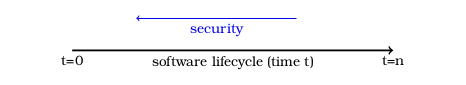
\includegraphics{../images/shift_left.png}
\caption{Shifting Left}
\label{shift}
\end{figure}

\section{Zero Trust}

\justify{}
Starting from the assumption that all the computers and networks are inherently unsafe and/or already compromised, the 
Zero Trust model gives organizations a way of thinking when establishing a security posture.\cite{zerotrust} This premise,
while rather simple from the conceptual standpoint, can be anything but when it comes to application. The difficulties in
scaling this mindset up for larger organizations can quickly become anything but simple.

\section{Automation}

\justify{}
Consider what may happen when we want to apply the lessons from this book across a large environment made up of many hosts,
containers, pieces of application software, etc. It becomes a huge challenge for an operator to log in to each host or container
individually. Typing, or even cutting and pasting commands to keep things up and running properly, look at logs,
and so on becomes problematic. Creating shell scripts can be quite helpful, but is an outdated modality when we consider
the daunting size and complexity of the modern administrative domain.

\justify{}
This is a great use-case for automation. Automation\index{automation} is a way to provision and maintain some or many hosts
in a programmatic manner. Another desirable goal, and hopefully result of automation is to reduce the amount of
per-host interaction that comes with the work of administering systems. Automation is the force multiplier we use to achieve
scaling\index{scaling}. As DevSecOps practitioners, we are on a never-ending quest to achieve
scale-invariance\index{scale-invariance}, to borrow a term from the mathematical realm. That is to say, the tools we
build and processes we engender should work just as well for three machines as they do for three thousand.

\justify{}
Couple this principle with the explosive automation tooling ecosystem and you are on the path to doing more, better work in
less time with a smaller staff.

\section{Immutability}

\justify{}
There is obvious advantage of being able to quickly stand up new clones of our project to replace existing instances that
may be outdated, insecure, etc. The idea of immutability, in reference to software projects, is the degree to which something, 
our running project for example, can be changed. Immutability\index{immutability} is desirable, in that we wish to be able to
simply replace outdated instances of our project in their entirety. Upgrading and patching are inherently
problematic activities, high cost in terms of time, effort and money, that we have the technology to dissociate from. With
containerization, we can more easily achieve immutability across the software life cycle.

\section{Ephemerality}

\justify{}
Ephemerality\index{ephemerality} is the concept of something being inherently transitory in nature. For something to be
considered ephemeral, it can exist only briefly. Using immutable containers makes it easier to realize
infrastructure and hosts that are ephemeral. Rather than spending a great deal of time patching and upgrading systems as
we might in a traditional project stack that uses bare metal hosts or even virtual machines, we're going to
use Docker to create a new container in place of the old one. In other words, we're running our project in containers that
are immutable and ephemeral to the degree possible.

\section{Agile Methodologies}

\justify{}
The concept of Agile\index{agile} Software development is an expansive topic unto itself. Agile practices are commonly
regarded as an underpinning of a successful DevSecOps program. There are methodologies that can help with organizing our
work items, staying on task, and completion of work items in a timely manner. While people tend to have varying
opnionions on the desirability and efficacy of these methodolgies, there is no denying the
fact that they are prevalent among tech companies.

\subsection{The Backlog}
This is the place work items are captured and await triage and assignment to a developer.

\subsection{the Kanban Board}
This is typically a columnar layout of work, where each column is an indication of status and completeness.
For example, a backlog column on the left, and in-progress column in the middle, and a completed
column on the left. 
